
\subsection{Iteración 1}

En esta iteración se han diseñado todos los escenarios en los que se desarrolla el proyecto.  El primer paso es decidir como se conectarán los escenarios entre sí. 

La primera opción consiste en mantener cada escenario aislado del resto, haciendo que el jugador comience en el principal y sea transportado al escenario correspondiente a cada prueba cuando vaya a realizarla, siendo transportado de nuevo al escenario principal al completarla. Esta aproximación permite una mayor diferenciación y caracterización de cada escenario, pero puede resultar poco inmersiva ya que el jugador se ve transportado constantemente sin importar sus acciones.

La segunda opción mantiene todos los escenarios unidos entre sí en todo momento, haciendo que los escenarios de las pruebas formen parte del principal, esto aumenta enormemente la inmersión de usuario ya que todos los elementos del juego están a la vista y no hay movimientos de cámara ni posición ajenos al jugador. Con este enfoque se consigue más realismo y al mismo tiempo se reduce el tamaño y la carga de trabajo asociada a cada escenario, ya que las pruebas no necesitarán un entorno completo, si no que se reutiliza gran parte del escenario principal. 

Finalmente, por los motivos ya expuestos, se decide utilizar la segunda opción y crear un escenario principal que contenga diferentes partes para cada prueba.

Este proyecto toma prestadas muchas ideas y conceptos de los concursos televisivos, por lo que son una fuente de inspiración ideal para la estética y el diseño de los escenarios (véanse figuras \ref{fig:E3_ahoraCaigo} y \ref{fig:E3_atrapaMillon}).

\begin{figure}
  \centering
    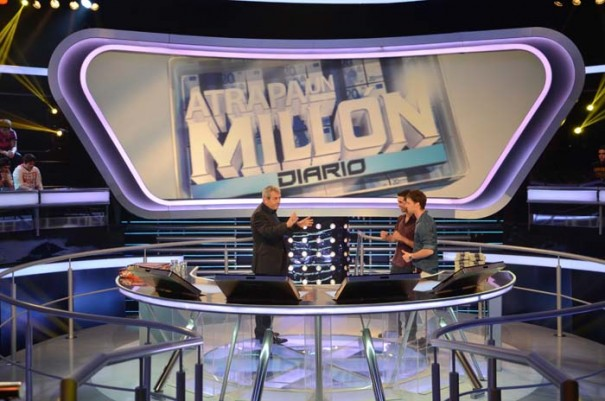
\includegraphics[width=0.7\textwidth]{04.Desarrollo/03.Entrega3/01.Iteracion3_1/00.Figuras/01.atrapa_un_millon.jpg}
    \caption{Plató del programa de televisión 'Atrapa un millón'. \cite{AI_img_atrapaMillon}}
    \label{fig:E3_atrapaMillon}
\end{figure}

\begin{figure}
  \centering
    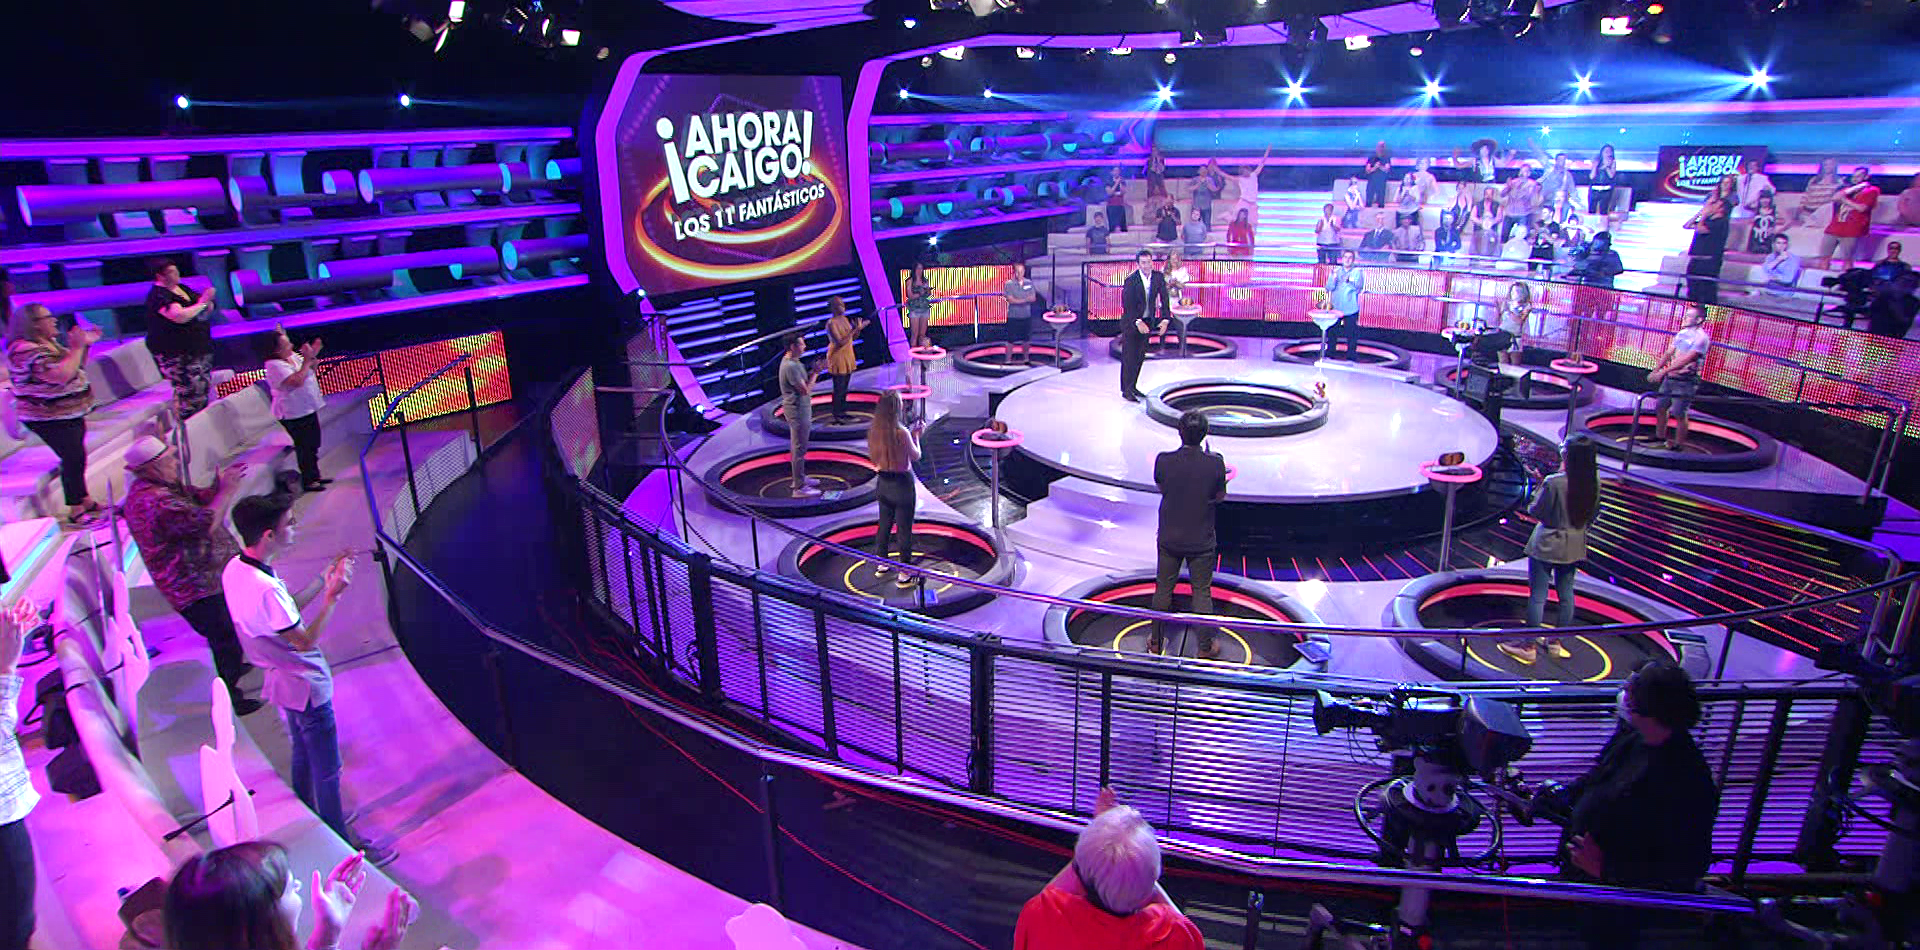
\includegraphics[width=0.7\textwidth]{04.Desarrollo/03.Entrega3/01.Iteracion3_1/00.Figuras/02.ahora_caigo.png}
    \caption{Plató del programa de televisión '¡Ahora caigo!'. \cite{AI_img_ahoraCaigo}}
    \label{fig:E3_ahoraCaigo}
\end{figure}




Como se muestra en las figuras \ref{fig:E3_escenarioArriba} y \ref{fig:E3_escenarioPerfil}, el escenario principal será circular, con el jugador situado en el centro. En los alrededores del habrá gradas con público (coloreadas de azul en las figuras), excepto en un trozo en el que se situará una pantalla gigante en la que se presentará información al jugador (rectángulo superior). En este caso, se ha designado una zona del escenario que es intercambiable (rayada en negro en las figuras), y en dicha zona aparecerá el escenario adecuado para cada prueba subiendo desde el suelo hasta la posición del jugador de forma similar a algunos elevadores en escenarios de espectáculos. Finalmente, la zona verde en las figuras contendrá elementos típicos de un plató de televisión como focos y altavoces, y su objetivo es encuadrar la zona donde transcurren las pruebas y se da información importante al jugador.


\begin{figure}
  \centering
    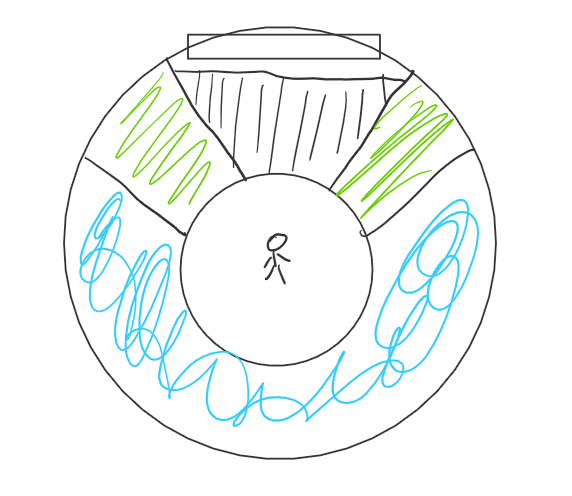
\includegraphics[width=0.5\textwidth]{04.Desarrollo/03.Entrega3/01.Iteracion3_1/00.Figuras/03.boceto_escenario_arriba.png}
    \caption{Boceto de la vista superior del escenario principal. En azul la zona de público, en verde la zona de atrezo, en negro la parte intercambiable para las pruebas.}
    \label{fig:E3_escenarioArriba}
\end{figure}

\begin{figure}
  \centering
    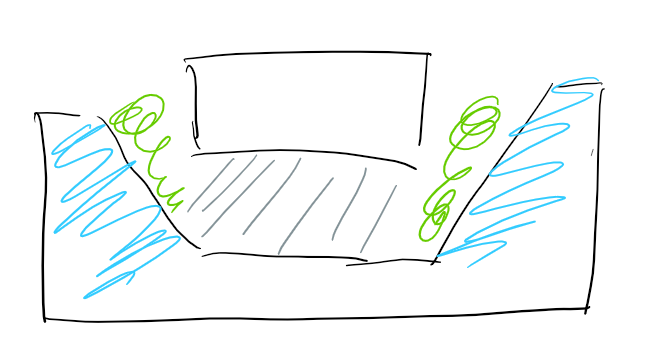
\includegraphics[width=0.5\textwidth]{04.Desarrollo/03.Entrega3/01.Iteracion3_1/00.Figuras/04.boceto_escenario_perfil.png}
    \caption{Boceto de la vista de perfil del escenario principal. En azul la zona de público, en verde la zona de atrezo, en negro la parte intercambiable para las pruebas.}
    \label{fig:E3_escenarioPerfil}
\end{figure}

Para la zona intercambiable del escenario que contendrá los distintos decorados, se ha buscado llenarla de objetos y atrezo relacionado con la prueba correspondiente, de forma que, al comenzar una prueba, aparecerá desde abajo todo el decorado y objetos necesarios para realizar dicha prueba. Tras finalizar la prueba, el escenario vuelve a su configuración original. Por tanto, solo es necesario diseñar un trozo pequeño del escenario para cada tipo de prueba.

Por lo general, las pruebas se pueden dividir en dos según el uso de su escenario: las que utilizan la pantalla principalmente y el resto es decoración, y las que utilizan los objetos virtuales del escenario como parte de la prueba y la pantalla sirve de decoración.


\subsubsection{Pruebas de pantalla}

Estas son las pruebas que utilizarán principalmente la pantalla y el resto del escenario contendrá objetos decorativos acordes con el tipo de prueba. La prueba de baile (figura \ref{fig:E3_baile}) utiliza la pantalla para mostrar al jugador los movimientos que tiene que realizar en cada momento, en este caso el escenario contendrá objetos como instrumentos musicales, tocadiscos, o una persona bailando.

\begin{figure}
  \centering
    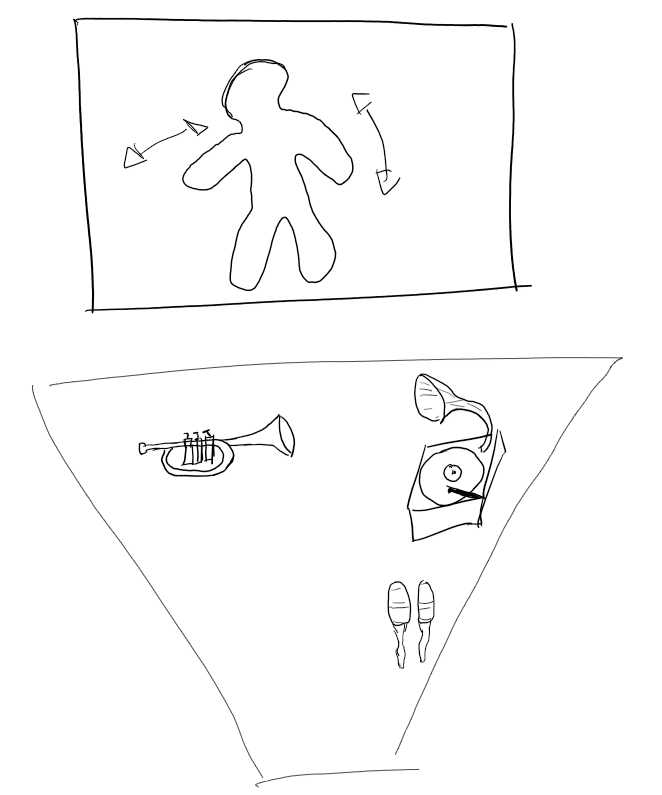
\includegraphics[width=0.5\textwidth]{04.Desarrollo/03.Entrega3/01.Iteracion3_1/00.Figuras/05.baile.png}
    \caption{Boceto del escenario para la prueba de baile.}
    \label{fig:E3_baile}
\end{figure}

La prueba de turismo también es de este tipo. En la pantalla de muestra una imagen de un monumento o lugar famoso que el jugador debe descubrir mientras que el resto del escenario se llena con objetos referentes a los viajes, como se muestra en la figura \ref{fig:E3_turismo}.

\begin{figure}
  \centering
    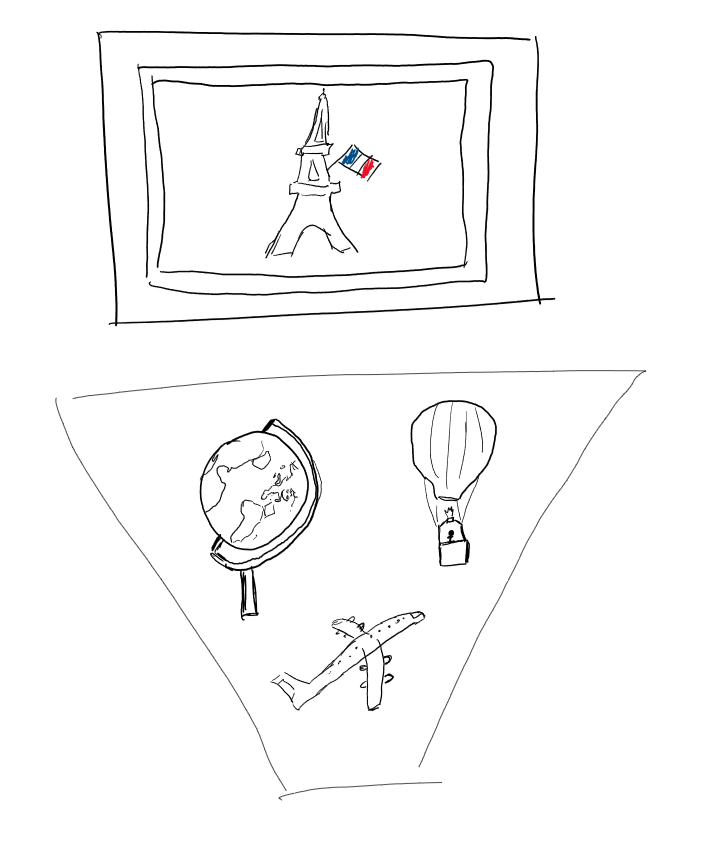
\includegraphics[width=0.5\textwidth]{04.Desarrollo/03.Entrega3/01.Iteracion3_1/00.Figuras/06.turismo.png}
    \caption{Boceto de la decoración para la prueba de turismo. En la pantalla una imagen de la torre Eiffel, con decorado de viajes: avión, globo terráqueo y globo aerostático.}
    \label{fig:E3_turismo}
\end{figure}


En las pruebas de situaciones y descripciones se sigue el mismo diseño, en la pantalla se muestra una imagen o situación que el jugador debe comentar. Pero estás pruebas podrían ser del segundo tipo y usar el escenario en lugar de la pantalla si la situación a describir es una que se puede representar con objetos virtuales animados en lugar de una foto o video en la pantalla.

La prueba de adivinar la canción es un caso especial, ya que, tratándose de sonido, no es necesario el uso de la pantalla, pero de igual forma se puede decorar el escenario como se muestra en la figura \ref{fig:E3_cancion}.

\begin{figure}
  \centering
    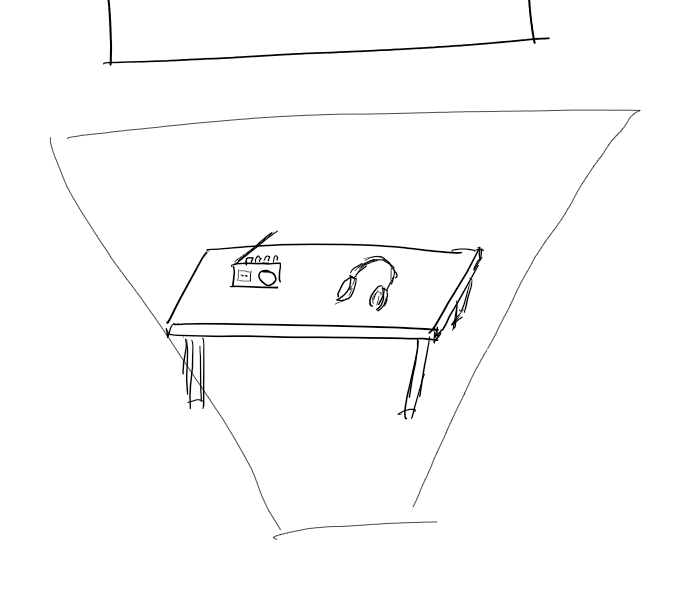
\includegraphics[width=0.5\textwidth]{04.Desarrollo/03.Entrega3/01.Iteracion3_1/00.Figuras/07.cancion.png}
    \caption{Boceto de la decoración para la prueba de adivinar la canción.}
    \label{fig:E3_cancion}
\end{figure}

Finalmente, en la prueba de superposición de objetos, se mostrará una imagen en la pantalla y el jugador tendrá que discernir de qué objetos se trata. Para facilitar esta tarea es sería posible que en el escenario aparecieran varios objetos virtuales, entre ellos los que se encuentran superpuestos en la imagen de la pantalla.



\subsubsection{Pruebas de escenario}

Estas son aquellas pruebas que dependen de los objetos del escenario y requieren su interacción para ser completadas, dejando a la pantalla el papel de decoración.

La prueba de figuras, en la que el usuario debe adoptar una posición que se le muestra antes de que se acabe el tiempo, utiliza un objeto que imita a un recortable de cartón o espantapájaros de una silueta posando. Dicha silueta se moverá hacia el usuario y este debe haber adoptado la posición correcta cuando la silueta llegue al jugador. El funcionamiento de esta prueba aparece bocetado en la figura \ref{fig:E3_figuras}.


\begin{figure}
  \centering
    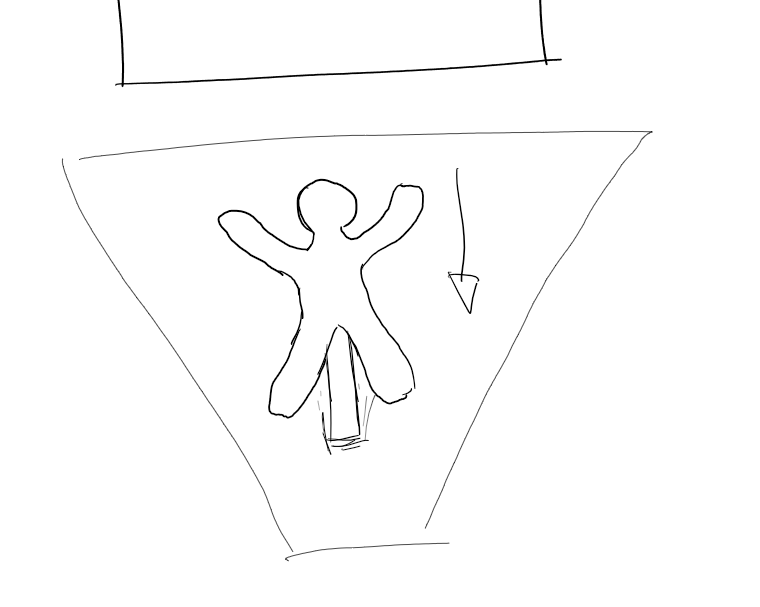
\includegraphics[width=0.5\textwidth]{04.Desarrollo/03.Entrega3/01.Iteracion3_1/00.Figuras/08.figuras.png}
    \caption{Boceto para la prueba de figuras, con una silueta acercándose al jugador.}
    \label{fig:E3_figuras}
\end{figure}

Para la prueba de objetivos, en la que el jugador debe tocar objetos que se mueven hacia él, el escenario utilizado solo contendrá dichos objetos en movimiento, como se pueden ver en el boceto de la figura \ref{fig:E2_objetivos}.



Para la prueba de asociación de sonidos únicamente se presenta ante el jugador una mesa en la que aparece un grupo de distintos objetos y el jugador debe seleccionar cual está produciendo el sonido mediante botones colocados frente a cada objeto (figura \ref{fig:E3_sonidos}). De forma similar, la prueba de agrupación de objetos también utiliza solo una mesa con un grupo de objetos, en este caso tiene también dos zonas donde agrupar los objetos por sus categorías (figura \ref{fig:E3_agrupacion}).

\begin{figure}
  \centering
    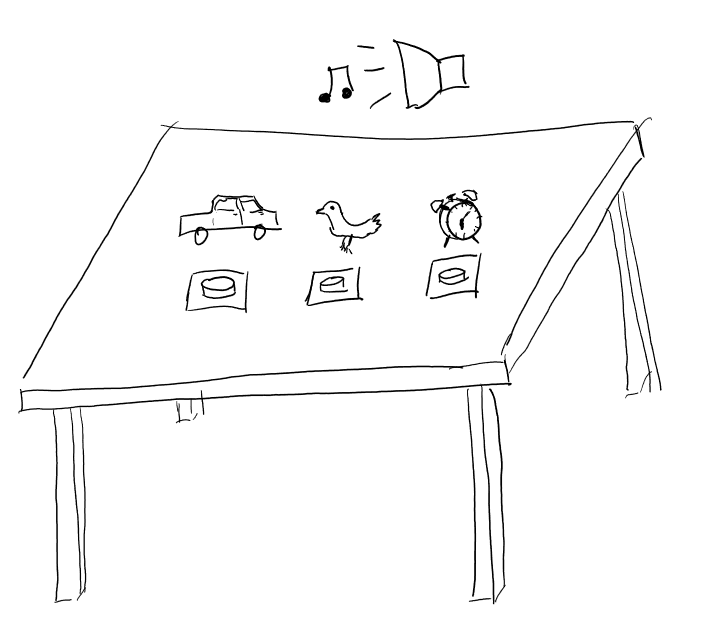
\includegraphics[width=0.5\textwidth]{04.Desarrollo/03.Entrega3/01.Iteracion3_1/00.Figuras/09.sonidos.png}
    \caption{Boceto con la mesa para la prueba de asociación de sonidos. Presenta distintos objetos con botones que corresponde a cada uno.}
    \label{fig:E3_sonidos}
\end{figure}

\begin{figure}
  \centering
    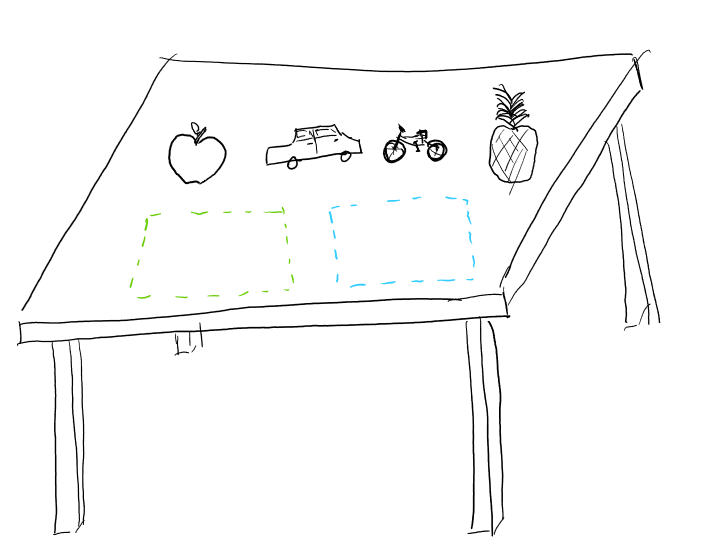
\includegraphics[width=0.5\textwidth]{04.Desarrollo/03.Entrega3/01.Iteracion3_1/00.Figuras/10.agrupacion_objetos.png}
    \caption{Boceto para la prueba de asociación de objetos, mostrando dos zonas (verde y azul) para la clasificación de los objetos.}
    \label{fig:E3_agrupacion}
\end{figure}


Por último, está la prueba de localización de sonidos, en este caso el escenario a utilizar es el propio escenario principal, ya que la prueba consiste en colocar una fuente de sonido en un punto del espacio y que el jugador se gire hasta encontrarla. De este modo se puede aprovechar el amplio espacio del escenario para colocar la fuente como se ve en la figura \ref{fig:E3_localizacionSonido}.

\begin{figure}
  \centering
    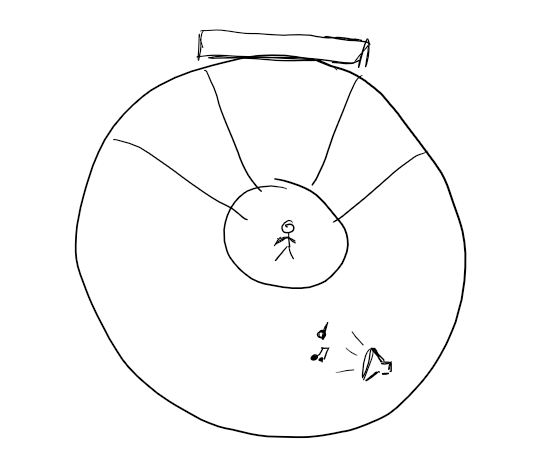
\includegraphics[width=0.5\textwidth]{04.Desarrollo/03.Entrega3/01.Iteracion3_1/00.Figuras/11.localizacion_sonido.png}
    \caption{Boceto de la vista cenital del escenario principal, mostrando una posible colocación de la fuente de sonido para la prueba de localización de sonidos.}
    \label{fig:E3_localizacionSonido}
\end{figure}

